\chapter{Introducing heterogeneities}
\label{chp:chp4}

In this chapter, we will consider how to mark, remove, and mesh
different regions of the brain and its environment based on
{\freesurfer} segmentations. We will
\begin{itemize}
\item
  create hemisphere meshes differentiating between gray and white matter;
\item
  create hemisphere meshes without ventricles;
\item
  create brain meshes by combining the two hemispheres;
\item
  map parcellations onto brain meshes;
\item
  locally refine parcellated brain meshes.
\end{itemize}

\section{Hemisphere meshing with gray and white matter}
\label{sec:chp4:tools:gray-white}

Gray and white matter differ substantially in their
characteristics. These differences may often be represented in
mathematical models and simulations by differing material
properties. For instance, denoting $\Omega_g$ and $\Omega_w$ by the
domains occupied by gray and white matter respectively, we may want to
consider heterogeneous diffusion tensors in~\eqref{eq:diffusion}
e.g.~such that
\begin{equation}
  \label{eq:K}
  K = K(x) = \left \{
    \begin{matrix}
      K_g & \quad x \in \Omega_g, \\
      K_w & \quad x \in \Omega_w 
    \end{matrix}
    \right .
\end{equation}
where $K_g$ and $K_w$ take different values, and where $K_g$ may be
scalar- and $K_w$ be tensor-valued. In order to represent fields such
as $K$ in numerical simulations, it is useful to carry the information
about gray and white matter from the MR images into the meshes. To
introduce the basic concepts of differentiating brain regions, we will
here create a computational mesh of the left hemisphere, as in
Chapter~\ref{chp:chp3}, but now conforming to the gray and white
matter regions. In short, we will
\begin{itemize}
\item
  create STL files from the pial and white FreeSurfer left hemisphere
  surfaces, and
\item
  create a mesh from these STL files conforming to interior interface
  between white and gray matter using \svmtk{},
\item
  with tags for different regions relative to the surfaces.
\end{itemize}

\subsection{Converting pial and gray/white surface files to STL}

Starting from the \freesurfer{} segmentation and using the book data
from \emp{freesurfer/ernie/surf/} as an example, we first convert the
left hemisphere pial surface (\emp{lh.pial}) and gray-white interface
surface (\emp{lh.white}) files to STL format (as described in
Chapter~\ref{sec:chp3:surfaces}):
\terminal{\$ mris\_convert ./lh.pial pial.stl\\
\$ mris\_convert ./lh.white white.stl
}
\noindent We can now also improve the quality of the resulting surfaces as
discussed in
Chapter~\ref{sec:chp3:improved-volume-meshing}\footnote{We leave the
  precise code for this as an exercise to the reader. The resulting
  files could be called \emp{lh.pial.smooth.stl} and
  \emp{lh.white.smooth.stl}. For simplicity, we assume that the
  resulting pial and white surface STL files are (re)named
  \emp{lh.pial.stl} and \emp{lh.white.stl} in the following.}.

\subsection{Creating the gray and white matter mesh}

Given these two surfaces, we can create a volume mesh conforming to
the interior (gray-white) surface and with the white and gray regions
identified separately. We will use \svmtk{} for this task, and
demonstrate via a \svmtk{} code example. We will wrap the main
functionality in a Python function
\pythoninline{create\_gw\_mesh}. This function can then, for instance,
be called as:
\newpythonsnippet{chp4}{two-domain-tagged.py}{25}{28}
to take the two STL surface files from above as input and create a new
file \emp{ernie-gw.mesh} for the resulting volume mesh.

Our function first loads the two surfaces using \svmtk{}:
\newpythonsnippet{chp4}{two-domain-tagged.py}{0}{8}

\noindent We next create a tailored \svmtk{}
\pythoninline{SubdomainMap} object that represents a map between
regions defined by surfaces and tags. This map is defined by
(repeated) calls to \emp{smap.add} with a string representing the
region and an integer representing the tag as arguments. The (binary)
string is a sequence of 0s and 1s: the 0 denotes "outside" and 1 is
"inside".
\newpythonsnippet{chp4}{two-domain-tagged.py}{9}{14}

A \svmtk{} \pythoninline{Domain} object be constructed from the
ordered list of surfaces and the subdomain map:

\newpythonsnippet{chp4}{two-domain-tagged.py}{16}{19}

\noindent Note that the \pythoninline{Domain} object here links the
surfaces and the subdomain map. The order of the entries in the list
of surfaces is matched with the binary region strings in the subdomain
map. The string \pythoninline{"10"} with reference to the list
\pythoninline{[pial, white]} is interpreted as "inside pial" and
"outside white" and thus represents the region between the pial and
white surface i.e.~the gray matter. Similarly, the string
\pythoninline{"11"} with reference to the same list is interpreted as
"inside pial" and "inside white" and thus represents the region inside
the gray-white surface i.e.~the white matter. We will discuss the
\pythoninline{SubdomainMap} further in Chapter~\ref{chp4:subdomains}
below.

With \pythoninline{domain}, we can now create a volume mesh of
a suitable resolution and save it in the .mesh format (as we did in
Chapter~\ref{subsec:chp3:mesh-creation}):
\newpythonsnippet{chp4}{two-domain-tagged.py}{20}{24}

This script is also available as \emp{mri2fem/chp4/two-domain-tagged.py} in the
book scripts, and can be run from there as:
\terminal{\$ python two-domain-tagged.py}

\noindent As before, the resulting .mesh can be converted to different formats
using meshio. For instance, to convert to the Paraview-friendly .vtu format: 
\terminal{\$ meshio-convert ernie-gw.mesh ernie-gw.vtu}

We have used Paraview to visualize the tags associated with this mesh
in Figure~\ref{fig:chp4:ernie-tagged-twodomain-mesh}. We see that the
mesh cells associated with the gray matter region have the value 1,
while the cells associated with the white matter region have the value
2 -- as defined by our subdomain map.

\begin{figure}
  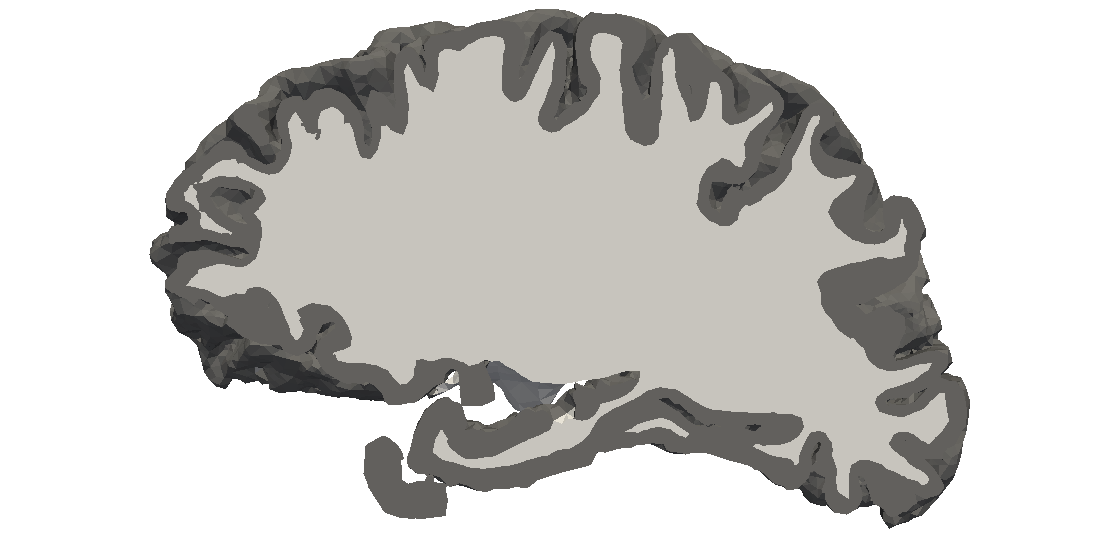
\includegraphics[width=0.49\textwidth]{./chapters/chp4/FIG/two-domain-tagged-a.png}
  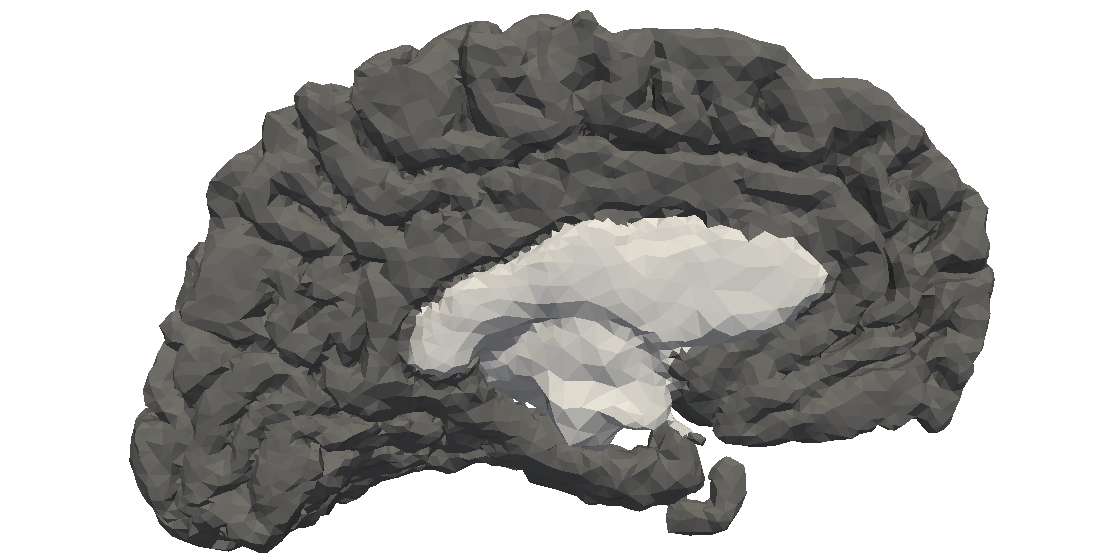
\includegraphics[width=0.49\textwidth]{./chapters/chp4/FIG/two-domain-tagged-b.png}
  \caption{Volume mesh of the left hemisphere conforming to the
    interior gray/white interface, and with the gray and white matter
    regions marked separately.}
  \label{fig:chp4:ernie-tagged-twodomain-mesh}
\end{figure}

\mer{@TBT: Did you make Figure 4.1? Could you improve the resolution of the mesh and the graphics? Maybe also it would be nice to show the mesh cells in one of the regions?}

As a side-note, we observe that the ventricles have been labeled as
white matter (see Figure \ref{fig:chp4:ernie-tagged-twodomain-mesh},
right) as the ventricles are positioned "inside" the gray-white
interface surface. Removing the ventricles from our computational mesh
is the topic of Chapter~\ref{sec:chp4:tools:remove-vent}.

\subsection{More about defining \svmtk{} subdomain maps}  
\label{chp4:subdomains}

To give more detail about the \svmtk{} feature
\pythoninline{SubdomainMap}, we consider another, more involved
example. We now suppose that we have four surfaces: a left pial
surface, a right pial surface, the whole white matter surface and a
surface enclosing the ventricles. A schematic of this set-up is
illustrated in Figure~\ref{fig:chp4:smap-example}. Now, let's see how
we can tag all the tetrahedra of the ventricles.
\begin{figure}[t]
  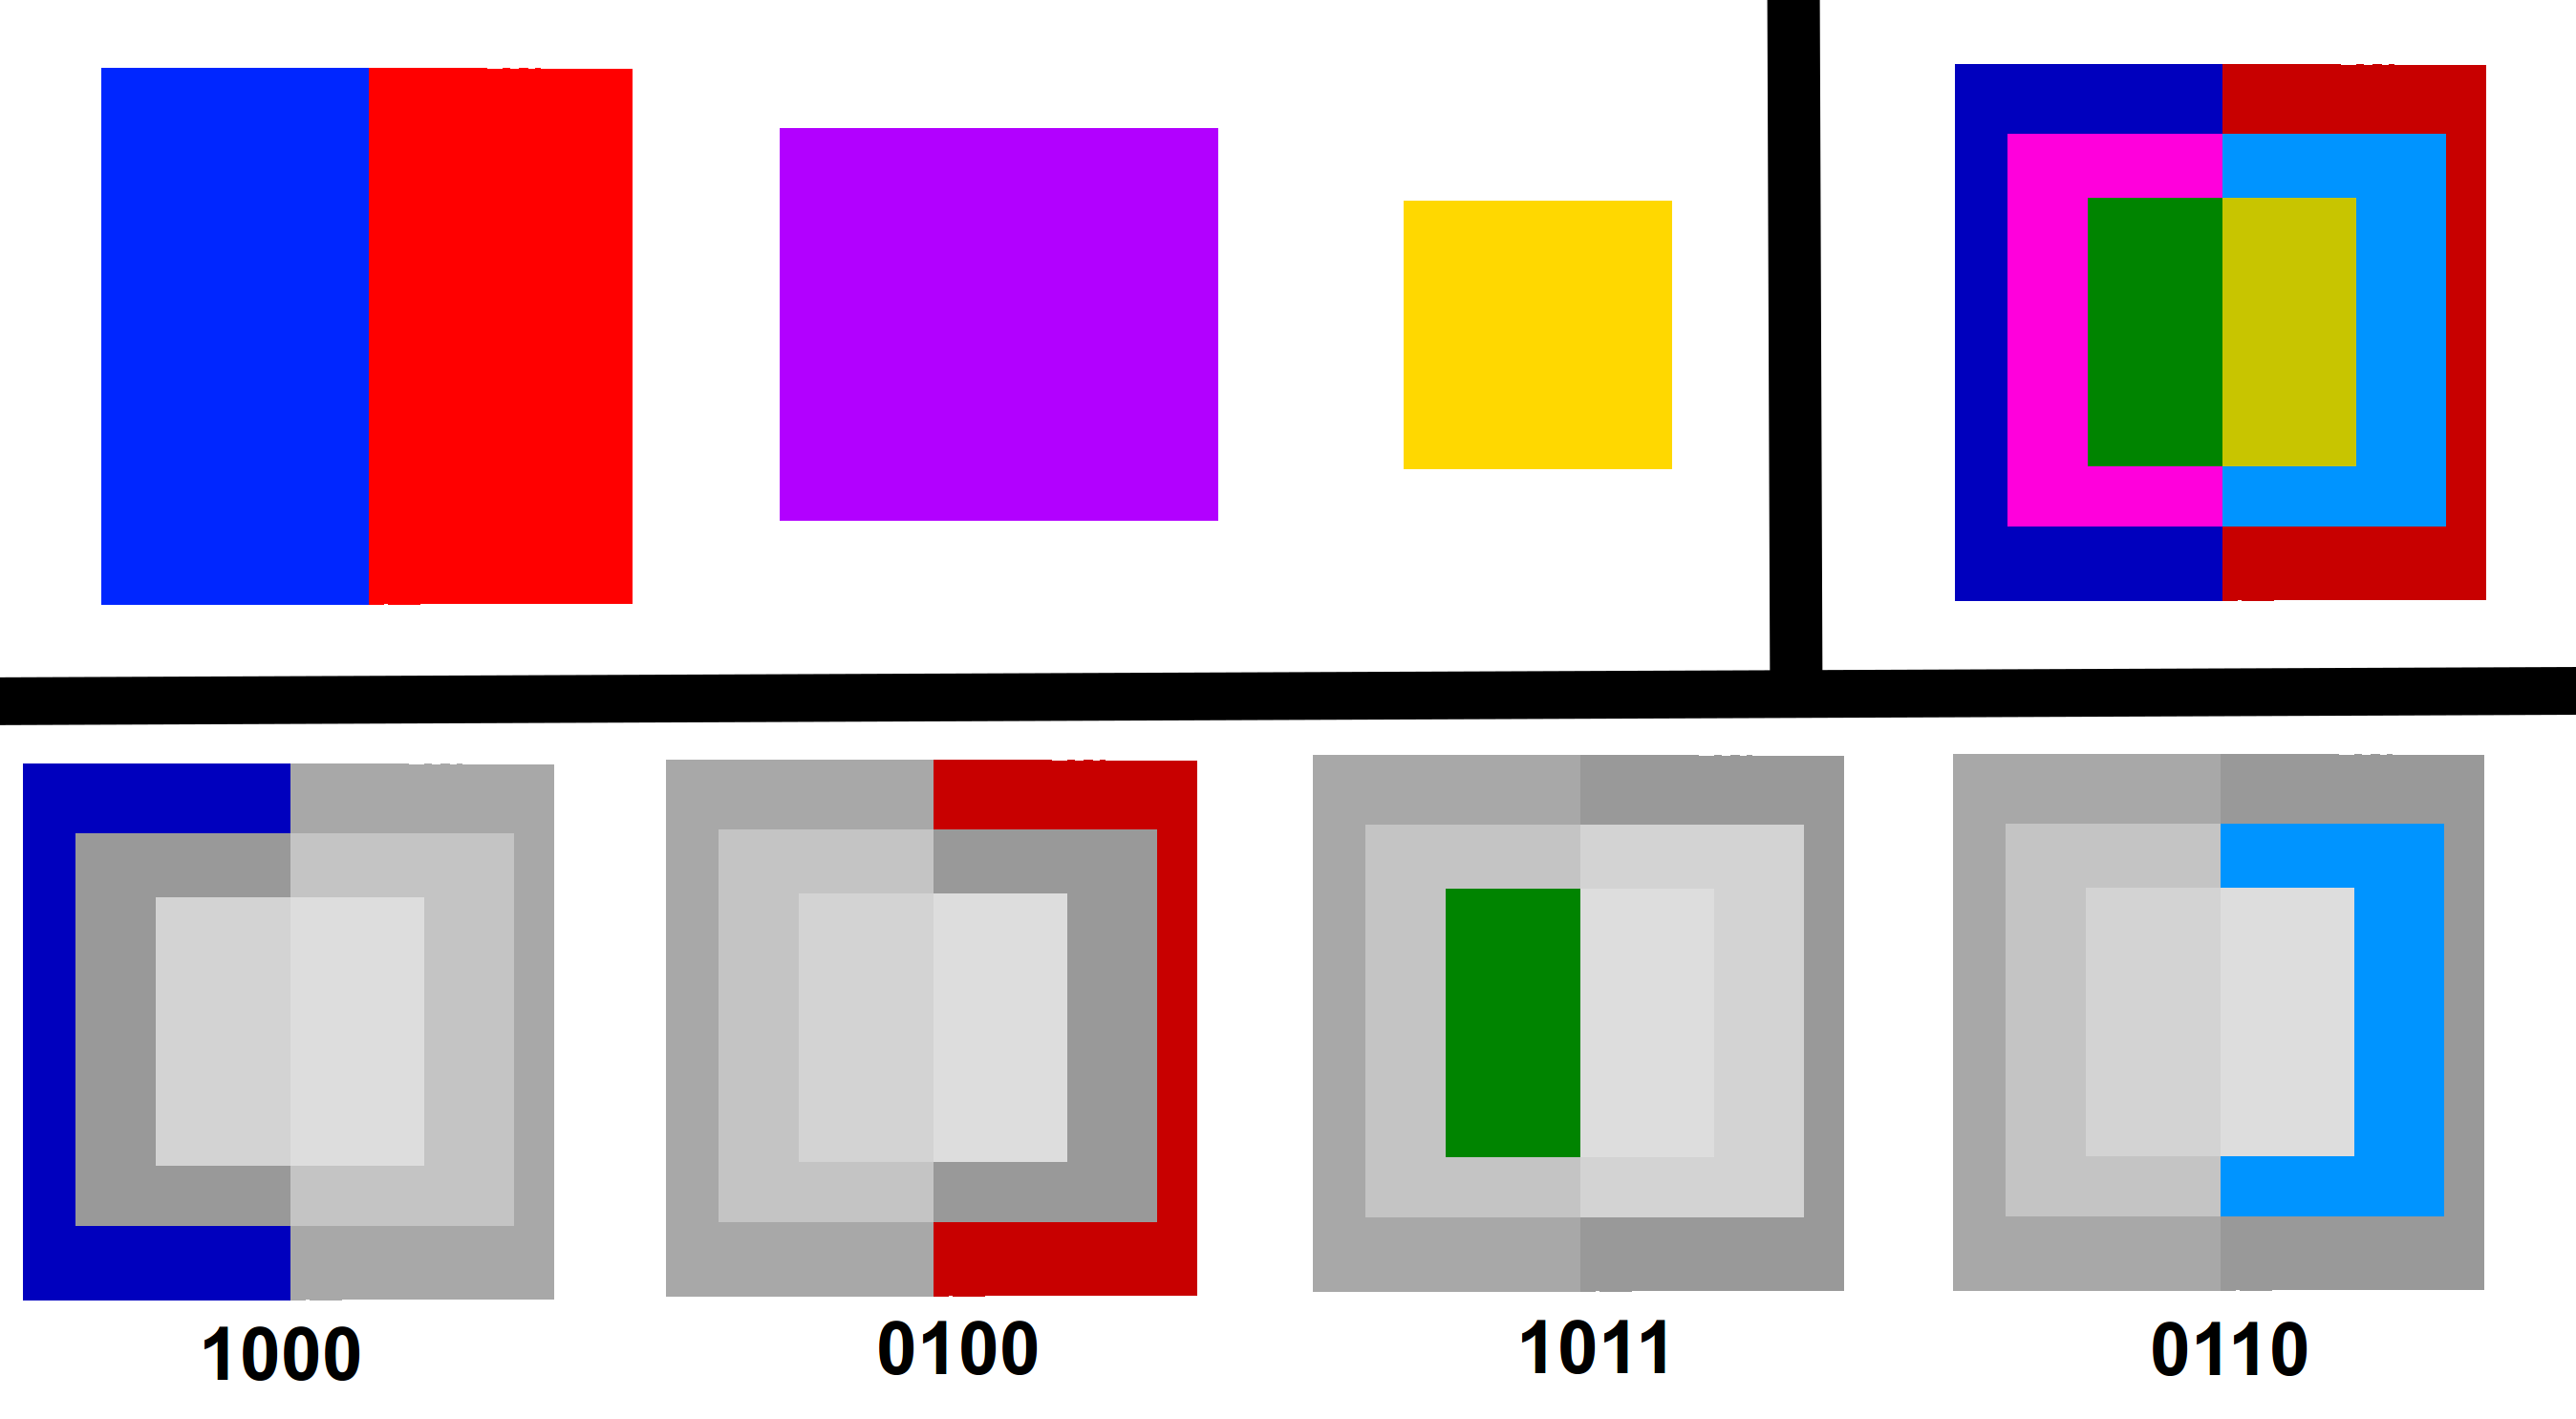
\includegraphics[width=0.95\textwidth]{./chapters/chp4/FIG/dot.png}
  \caption{The upper left panel shows colored squares, each
    schematically representing a domain enclosed by a surface. The
    left hemisphere is blue, the right hemisphere is red, the white
    matter is purple and the ventricles are yellow, and their bounding
    surfaces are given in this order. The upper right panel shows the
    combination of each colored square. The bottom panel shows four
    different subdomains and its corresponding bit-string. The left
    image "1000" denotes the volume that is within the left
    hemisphere, but not within the right hemisphere, white matter or
    ventricles; hence the gray matter of the left hemisphere. The
    "0100" is completely analogous for the right hemisphere. Then
    "1011" refers to the surface that is within the left hemisphere
    and within both white and ventricles; hence the left
    ventricle. Finally, "0110" represents the white matter of the
    right hemisphere.  }
\label{fig:chp4:smap-example}
\mer{I like this figure a lot, but I do not like the thick black
  lines. Could we remove those? We could alternatively use (a), (b),
  (c).}
\end{figure}

To represent the subdomains, assuming that \pythoninline{lpial, rpial,
  white} and \pythoninline{ventricles} exist as
\pythoninline{svmtk.Surface}s, we could use the following sample code
\begin{python} 
surfaces = [lpial, rpial, white, ventricles]
smap = svmtk.SubdomainMap()
\end{python}
To mark all the tetrahedra in the ventricles in the left hemisphere
with the tag value 6, we need to identify the placement of the left
ventricles within the ordered list of surfaces. Note that the STL
surface format includes information about the orientation of the
surfaces via the surface normals: thus each surface has an orientation
with an inside and an outside direction. The ventricles in the left
hemisphere are inside the left pial surface, outside the right pial
surface, inside the gray-white matter surface and inside the
ventricular surface, resulting in the bit-string "1011". We could thus
call \pythoninline{smap.add} as
\begin{python}
smap.add("1011", 6)
\end{python}
Similarly, we can tag the ventricle volume within the right pial
surface by
\begin{python}
smap.add("0111", 6)
\end{python}
Finally, we can tag the ventricular volume at the intersection of the
left and right pial surfaces via
\begin{python}
smap.add("1111", 6)
\end{python}
Indeed, tagging the entire ventricular volume in this manner requires that we add all
three of the lines above.

Finally, we remark that {\svmtk} also allows for marking several
domains at once:
\begin{python}
smap.add("10*", 6)
\end{python}
will mark all underlying domains, i.e., in this case "1000", "1001", "1010", and "1011".   
\mer{So, could we just have done  smap.add("$\ast$1", 6)?}

\section{Separating the ventricles from the gray and white matter}
\label{sec:chp4:tools:remove-vent}

The volume meshes created in Chapter~\ref{chp:chp3}, and the
hemisphere mesh illustrated in
e.g.~Figure~\ref{fig:chp4:ernie-tagged-twodomain-mesh} include the
ventricles as part of the white matter. As the physics of the
fluid-filled ventricles and the soft but solid brain cerebrum may be
very different, removing the ventricles from the hemisphere volume is
a useful operation. Here, we demonstrate (i) how to use {\freesurfer}
to extract and postprocess the ventricular surface; and (ii) how to
remove the resulting ventricular volume from the cerebrum.

\subsection{Extracting a ventricular surface from MRI data}
\label{sec:chp4:tools:remove-vent:extraction}  

We will extract the ventricle surface(s) from our T1 MRI data via
{\freesurfer}. Extracting a ventricular surface representation is
relatively straight-forward, while extracting a high-quality surface
representation may be more involved. We therefore introduce tools and
utilities of increasing complexity here.

\subsubsection*{Segmentations and parcellations: a sneak peek}
\index{segmentation}
\index{parcellation}
Recall that \freesurfer's \emp{recon-all} generates a number of
surface and volume files (see
e.g.~Chapter~\ref{sec:chp3:surfaces}). In particular, the
\freesurfer{} generated \emp{mri/} directory includes volume-based
data, such as T1-weighted images, segmentations and
parcellations. These volume files have the extension \emp{mgz}, and
the segmentations and parcellations can be identified by the base
filename. For instance, the file \emp{aseg.mgz} stands for automatic
segmentation, and the file \emp{wmparc.mgz} stands for white matter
parcellation. The parcellation will split the segmentation into finer
regions, e.g.~the cortical gray matter will be divided into 35 regions
for each hemisphere. We can use the segmentation or the parcellation
files to construct the surface of the ventricular volume. 

The segmentations can be inspected using e.g. Freeview. To
exemplify, we use the \freesurfer{} generated files from our data set
at \emp{freesurfer/ernie/mri}, and visualize the \emp{aseg.mgz}
file:
\terminal{\$ cd freesurfer/ernie/mri \\ \$
  freeview -{}-colormap lut -{}-v aseg.mgz}

\noindent The list in the left hand pane of the Freeview window shows
the segmentation tags, i.e values associated with different brain
regions. Alternatively, letting the pointer hover over a voxel will
cause the corresponding region tag and name to appear in the bottom
right corner. For instance, the left hippocampus has tag 17, while the
4th ventricle has tag 15. We will look more into segmentations and
parcellations in Chapter~\ref{sec:import-freesurfer-parcellation},
including a visualization in Figure~\ref{fig:chp4:freesurfer-parc}.

\subsubsection*{Extracting and binarizing voxel-based information}

The {\freesurfer} command \emp{mri\_binarize} is used to extract and
mark voxels that contain a certain type of information such as a range
of signal values, or a collection of segmentation tags. The command
includes about 40 optional flags, all of which are described in
\terminal{\$ mri\_binarize -{}-help}

\noindent or via the FreeSurfer online
documentation~\cite{freesurfer-wiki}; we will focus on but a few of
these here.

The input file is given following the flag \emp{-{}-i}, and a volume
output file (\emp{.mgz}) is given following the flag \emp{-{}-o}. A
surface output file (\emp{.stl}) can be given, in addition to or
instead of the volume output, following the flag \emp{-{}-surf}. The
essential flag \emp{-{}-match}, followed by one or more integers, will mark
all voxels matching any of the given integer values. For instance, to
select all voxels from the 4th ventricle, we can use \emp{-{}-match
  15}. Alternatively, specific regions can also be identified by
designated flags, for instance:
\begin{itemize}
\item \emp{-{}-ventricles} marks voxels in the third and lateral ventricles, and in the choroid plexus
\item \emp{-{}-ctx-wm} marks voxels in the cerebral white matter 
\item \emp{-{}-gm} marks voxels in the gray matter  
\item \emp{-{}-subcort-gm} marks voxels in the subcortical gray matter, including the gray matter in the cerebellum and brainstem.  
\end{itemize}
These flags can be combined -- for example: 
\terminal{\$ mri\_binarize -{}-i aseg.mgz -{}-ventricles -{}-match 15 -{}-o v.mgz}

\noindent will mark the third and lateral ventricles (via the
\emp{ventricles} flag) and the fourth ventricle (with match value
15). In the output file, all the marked voxels will have the value 1
and the rest will be set 0. This can be changed by specifying the
output binvalue with the optional flag \emp{-{}-bin} followed by an
integer. The marked voxels will now have the selected bin value in the
output. The surface output flag \emp{--surf} is often used together
with the flag \emp{-{}-surf-smooth} followed by an integer determining
the number of smoothing iterations on the output surface. 

To extract the ventricular surface from our white matter parcellation,
we define a customizable bash script (\emp{extract-ventricles.sh}). We begin by defining the input and output file names:
\lstinputlisting[style=bashStyle,firstline=1,lastline=5]{mri2fem/mri2fem/chp4/extract-ventricles.sh}

\noindent To extract a surface file of the ventricular system, we call
\emp{mri\_binarize} with the input filename (in \emp{input}), the \emp{--ventricles} flag, additional tags given by \emp{matchval}, and a number of smoothing iterations:
\lstinputlisting[style=bashStyle,firstline=47,lastline=51]{mri2fem/mri2fem/chp4/extract-ventricles.sh}

\noindent Prior to this call, we allow for including the fourth
ventricle and aqueduct by setting the \emp{matchval} variable, and
we set the \emp{num\_smoothing} iterations:
\lstinputlisting[style=bashStyle,firstline=7,lastline=15]{mri2fem/mri2fem/chp4/extract-ventricles.sh}

\noindent It is suggested to set \emp{num\_smoothing} to an
integer value between $1$ and $5$. The resulting ventricular surfaces
with 0 and 5 smoothing iterations, both including the fourth
ventricle, are shown in
Figure~\ref{fig:chp4:ernie-ventricles-smoothing-example}.
\begin{figure}
  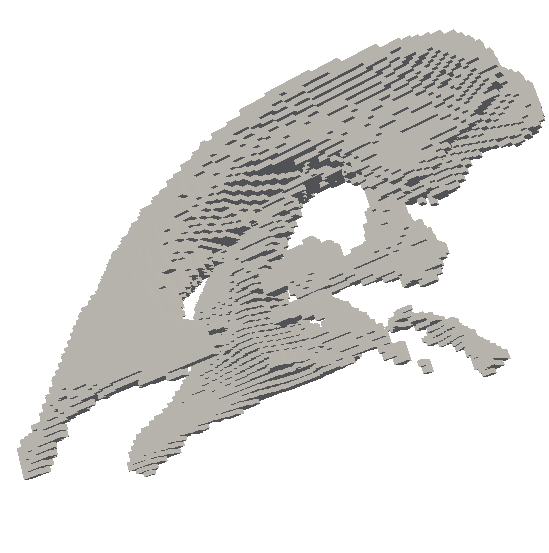
\includegraphics[width=0.49\textwidth]{./chapters/chp4/FIG/ernie-vent-0smooth.png}
  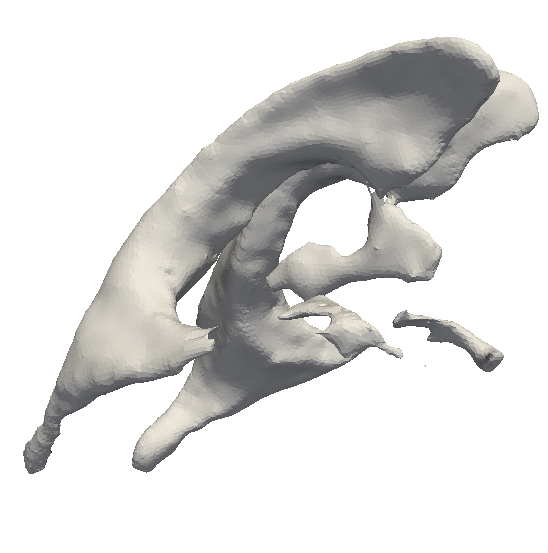
\includegraphics[width=0.49\textwidth]{./chapters/chp4/FIG/ernie-vent-5smooth.png}
  \caption{Ventricular surfaces, including the fourth ventricle,
    extracted and generated by \freesurfer{} from MRI images. No
    smoothing of the output surface (left) and five smoothing
    iterations (right). Note the presence of disconnected regions.}
  \label{fig:chp4:ernie-ventricles-smoothing-example}
\end{figure}

In practice, the decision to include or discard the fourth ventricle
and aqueduct is data specific. The aqueduct may not be well resolved
in the MRI data on a patient-by-patient basis; if the aqueduct is not
visible in the data then keeping the fourth ventricle leads to a
ventricle system that is not connected, as
Figure~\ref{fig:chp4:ernie-ventricles-smoothing-example} indeed
shows. Moreover, if the we include the fourth ventricle and aqueduct,
one should take care with regard to the extent of the smoothing. 

\subsubsection*{Improving the morphology of the ventricular surface}

We can improve the morphology and connectedness of the extracted
ventricular surface by more advanced processing via the \freesurfer{}
utilities \emp{mri\_volcluster} and \emp{mri\_morphology}.
\begin{itemize}
\item
  \emp{mri\_volcluster} is used to identify clusters in a volume. A
  cluster is defined as a set of continuous voxels that satisfies a
  threshold criteria. The input file is given following the flag
  \emp{-{}-in}, \emp{-{}-thmin} gives a minimum threshold value,
  \emp{-{}-minsize} gives a minimal cluster volume (in
  mm$^3$). Different output flags are
  admissible~\cite{freesurfer-wiki}, including \emp{-{}-ocn} used to
  save the output volume file with sorted clusters, all voxels of
  largest cluster will be have the tag 1, second largest would have
  the tag 2 and so on.
\item
  \emp{mri\_morphology} is used to perform certain operations on
  volume files. There are 9 different operations, which includes open,
  close, dilate, erode and fill holes. We will illustrate how to use
  this function below for connecting the extracted domain by closing
  holes. 
\end{itemize}

Using these functions, we may extract an improved, higher quality
ventricular surface by removing apparently disconnected regions. Our
algorithm takes the following steps:
\begin{enumerate}
\item
  We extract the lateral and third ventricles into a separate volume
  file.
\item
  In this separate volume, we extract clusters of connected voxels -
  but only those above a minimal cluster size. As the average adult
  volume of cerebrospinal fluid in the ventricles is about 150
  mm$^{3}$, we set the threshold size to be around 100 mm$^3$.
\item
  We extract the largest of these clusters (thus ignoring the smaller,
  disconnected regions)
\item
  We close holes in the resulting volume as need be.
\item
  We extract the surface of the resulting volume, and smoothen it as
  need be.
\end{enumerate}
The corresponding continuation of our Bash script follows below. Note
how we output the clusters sorted by size using the argument
\emp{-{}-ocn} to \emp{mri\_volcluster}, and extract the largest
cluster by matching on 1 in the subsequent call to
\emp{mri\_binarize}. We allow for setting the number of closing
iterations \emp{num\_closing} and minimal largest cluster size
\emp{V\_min} as parameters. It is advised to set the number of closing
iterations relatively low (e.g.~to 1 or 2). Setting the number of closing
iterations too high can cause non-physiological connections in the
resulting ventricular surface.
\lstinputlisting[style=bashStyle,firstline=16,lastline=46]{mri2fem/mri2fem/chp4/extract-ventricles.sh}

\begin{figure}%\sidecaption
  \centering
  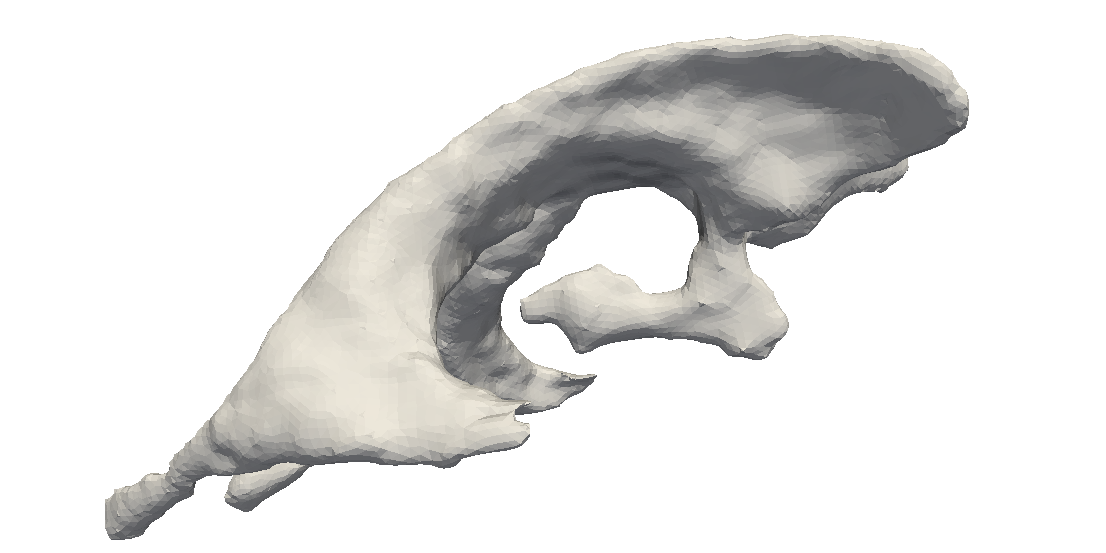
\includegraphics[width=0.95\textwidth]{./chapters/chp4/FIG/ernie-ventricles-final.png}
  \caption{High quality, connected and smooth ventricular surface
    (\emp{ernie-ventricles.stl}) extracted from MRI using
    \freesurfer{}. }
  \label{fig:chp4:ernie-ventricles-final}
\end{figure}
\noindent Figure~\ref{fig:chp4:ernie-ventricles-final} shows the ventricular
surface STL file generated by the above code but with
\emp{postprocess=true}, visualized in Paraview.

\subsection{Removing the ventricular volume}
\label{sec:chp4:tools:remove-vent:removal}  

In this section, we demonstrate how to remove a subvolume defined by
an enclosing surface. Though we will focus, here, on removing the
volume enclosed by the ventricle surface, as extracted in the previous
section, the general process will also work for any volume defined by
a closed surface STL file. The core idea is to use \svmtk{} to
generate tags for the different subvolumes in the domain and then
simply delete the volume corresponding to a specific tag.  

We assume that we have the left pial, gray/white matter, and ventricular
surfaces available as STL files. Again, we will wrap the main
functionality in a Python function
\pythoninline{create\_gwv\_mesh}. This function can then, for
instance, be called as:
\newpythonsnippet{chp4}{three-domain-tagged.py}{33}{35}

\noindent This code example is included in
\emp{mri2fem/chp4/three-domain-tagged.py}.

We first create \pythoninline{Surface}s from the surface STL files:
\newpythonsnippet{chp4}{three-domain-tagged.py}{1}{10}

\noindent We then tag different regions using a \pythoninline{SubdomainMap}: 
\newpythonsnippet{chp4}{three-domain-tagged.py}{12}{19}

\noindent As before, we create a tagged mesh (of a given resolution)
of the domain via the surfaces and the subdomain map:
\newpythonsnippet{chp4}{three-domain-tagged.py}{21}{24}

We can now, via a call to \svmtk{} \pythoninline{remove\_subdomain},
remove the mesh cells tagged as within the ventricles before saving
the mesh:
\newpythonsnippet{chp4}{three-domain-tagged.py}{26}{31}
Note that \pythoninline{remove\_subdomain} can also handle the removal of
multiple subdomains by giving a tuple of tags as input. The resulting
meshes, with and without ventricles removed, are shown in Figure
\ref{fig:chp4:tags-with-without-ventricles}.
\begin{center}
\begin{figure}
  %\imagetop{(a)}& \imagetop{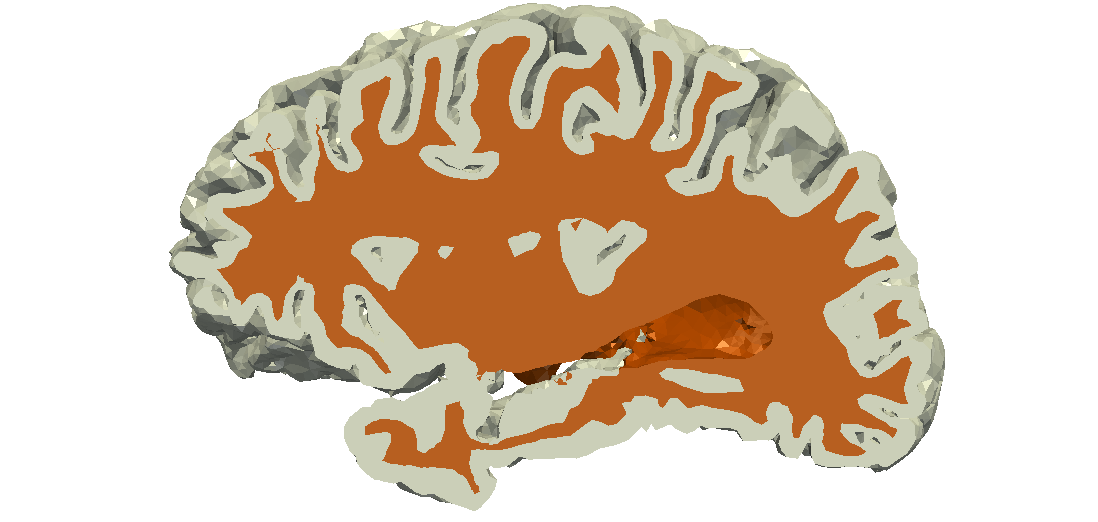
\includegraphics[width=0.49\textwidth]{./chapters/chp4/FIG/ernie-final-comp-a}} &
  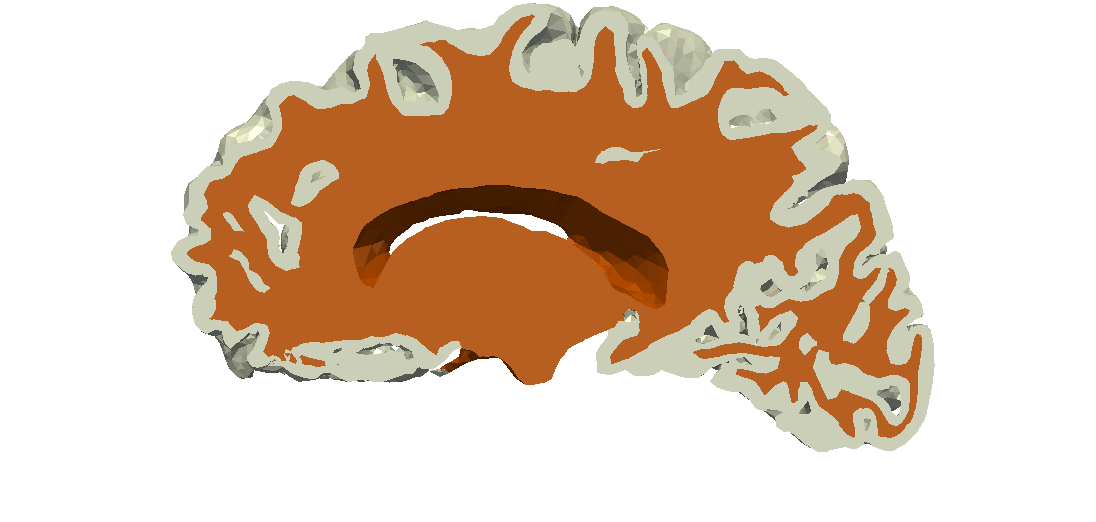
\includegraphics[width=0.49\textwidth]{./chapters/chp4/FIG/ernie-final-comp-b}
  %\imagetop{(c)}& \imagetop{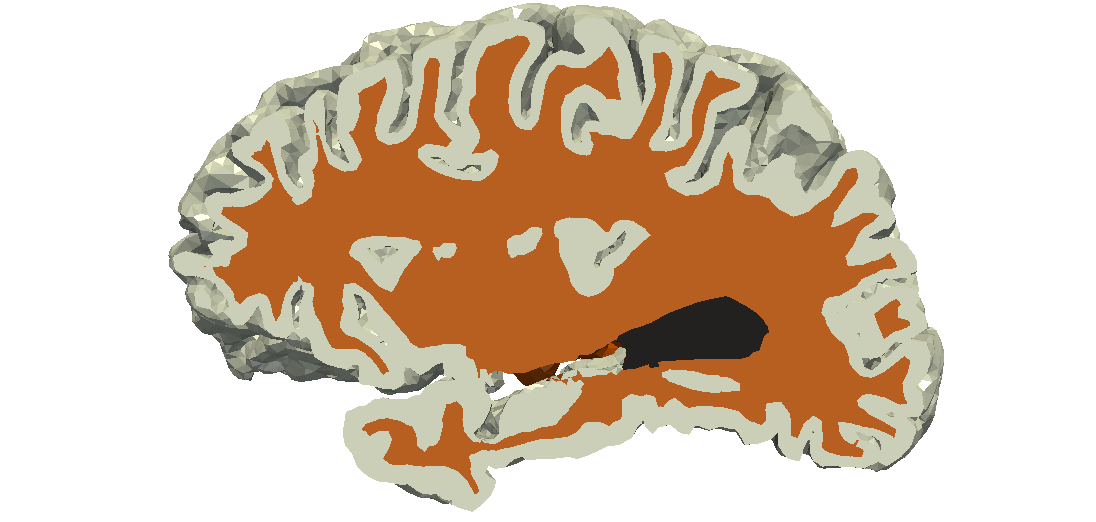
\includegraphics[width=0.49\textwidth]{./chapters/chp4/FIG/ernie-final-comp-c}} &
  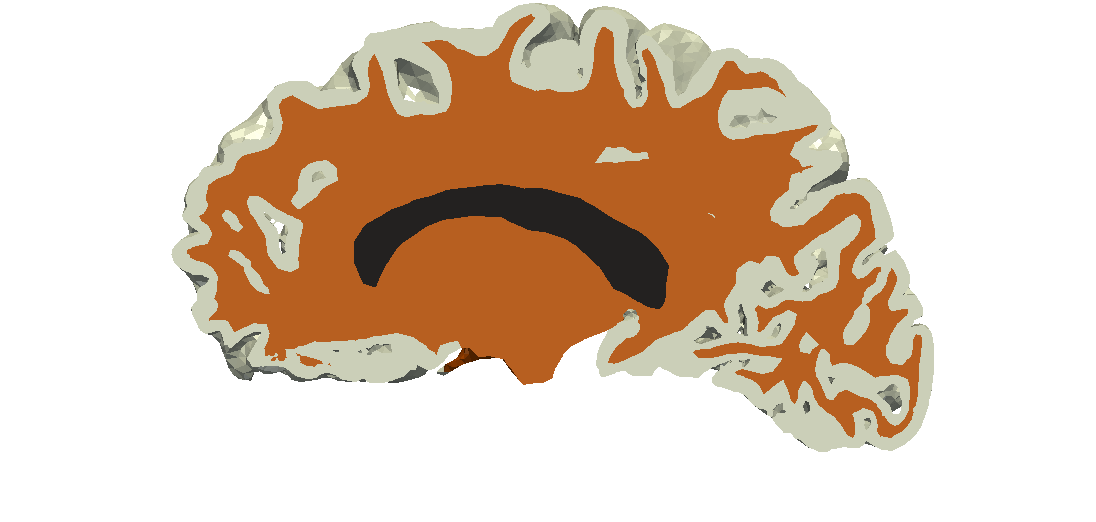
\includegraphics[width=0.49\textwidth]{./chapters/chp4/FIG/ernie-final-comp-d}
    \caption{Meshes of the left hemisphere (sagittal planes),
      conforming to the gray matter, white matter and ventricles, with
      ventricles removed (left) and ventricles not removed but marked
      in black (right).}
    \label{fig:chp4:tags-with-without-ventricles}
    \mer{Could we adjust the coloring of these plots? Perhaps with
      gray matter gray, white matter whiteish, and ventricles marked
      in a blue (CSF $\mapsto$ water $\mapsto$ blue)? Also, could we remove some of
      the surrounding white space? Also, do the ventricles extend
      all the way through the hemisphere (creating a channel)? If yes,
      why?}
    \mer{Which "version" of SVMTK is needed for remove\_subdomain?}
\end{figure}
\end{center}

\section{Bringing the hemispheres together}
\label{sec:chp4-left-right-tagged}

In this section, our aim is to create a mesh that includes both the
left and right hemispheres, with gray and white regions tagged, and
ventricular volume removed. We will combine the approaches of the
previous sections alongside together with \svmtk{} techniques for
working with the union of multiple surfaces. 

\subsection{Repairing overlapping surfaces}

\freesurfer{} generates the right and left hemisphere surfaces
separately. As a result, combining surfaces from different hemispheres
can create problems such as:
\begin{itemize}
\item the hemisphere surfaces overlap, creating bridges in the cortical gray matter;
\item the hemisphere surfaces do not overlap, creating gaps in the white matter. 
\end{itemize} 
We can consider this a combined problem, since we typically would want
to join the hemisphere surface via the white matter nerve tracts, but
avoid overlapping surfaces in the cortical gray matter. \svmtk{}
includes utilities for such addressing such challenges. In particular:
\begin{itemize}
\item
  \pythoninline{separate\_overlapping\_surfaces} can separate
  overlapping surfaces;
\item
  \pythoninline{separate\_close\_surfaces} can separate nearly
  overlapping surfaces;
\item 
  we may want create a single surface for the white matter, but the
  surfaces may only be partially overlapping due to smoothing. In this
  case, \pythoninline{union\_partially\_overlapping\_surfaces} offers
  improved features for the union of white matter surfaces.
\end{itemize}
The following code snippet illustrates sample usage of these functions.
\begin{python}
# Input Surfaces
rpial = svmtk.Surface("rh.pial.stl")
lpial = svmtk.Surface("lh.pial.stl")
rwhite = svmtk.Surface("rh.white.stl")
lwhite = svmtk.Surface("lh.white.stl")

# Create white matter surface as union of hemispheres
white = svmtk.union_partially_overlapping_surfaces(rwhite,
                                                   lwhite)

# Separate overlapping and close vertices between
# the left and right pial surfaces,
# but only outside the gray/white surface:
svmtk.separate_overlapping_surfaces(rpial, lpial, white)
svmtk.separate_close_surfaces(rpial, lpial, white) 
\end{python} 

\subsection{Combining surfaces to create a brain mesh}

We assume that left pial, left white, right pial, right white and
ventricular surface STL files have been extracted, converted and
possibly processed the processes described in the previous. Now, how
do we combine these to create a complete brain mesh? 

Again, we demonstrate via an \svmtk{} code example (with the complete
code included in \emp{mri2fem/chp4/fullbrain-five-domain.py}). We wrap
the main functionality in a Python function
\pythoninline{create\_brain\_mesh}. This function can then, for
instance, be called as:
\newpythonsnippet{chp4}{fullbrain-five-domain.py}{42}{45}

We begin by loading the \emp{Surface}s from the STL files. 
\newpythonsnippet{chp4}{fullbrain-five-domain.py}{0}{7}

We take the union of the left and right white surface to illustrate
possibility of combining surfaces:
\newpythonsnippet{chp4}{fullbrain-five-domain.py}{9}{15}
It is natural to ask whether we can do the same with the pial matter;
indeed, taking the union of the left and right pial surfaces is
possible. However, in general, whether or not one can successfully
mesh the joined surface, without further postprocessing, is data
specific.  There is a higher chance that the {\freesurfer}
segmentation process of the left and right pial MRI surface data can
lead to non-physical intersections; thus producing left and right pial
surface files that overlap and self-intersect when unioned together.
Self-intersections within a surface can then cause the meshing process
to fail. Likewise, one could simply work with all five surfaces
separately; this would lead to a more complicated tagging process with
the \emp{SubdomainMap} but alleviate difficulties that may arise when
computing the union two surface objects.

We continue by creating tags, a subdomain map, Domain and mesh, and leave the
option to remove the ventricles, as in previous examples:
\newpythonsnippet{chp4}{fullbrain-five-domain.py}{17}{40}

\begin{figure}
  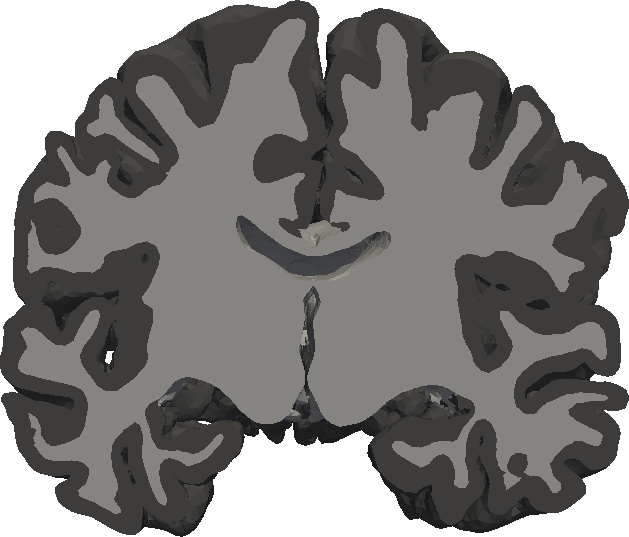
\includegraphics[width=0.49\textwidth]{./chapters/chp4/FIG/ernie-fullbrain-crop-a.png}
  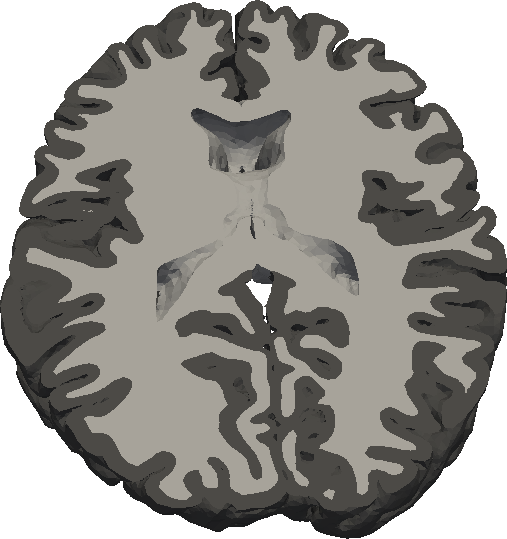
\includegraphics[width=0.49\textwidth]{./chapters/chp4/FIG/ernie-fullbrain-crop-b.png}
  \caption{Coronal (left) and axial (right) sections of full brain mesh 
    with gray and white matter marked and ventricles removed.}
  \label{fig:chp4:ernie-fullbrain-tagged}
  \mer{Can we make this look prettier? Alignment? Colors? Opacity? Angle of direction?}
\end{figure}
Running this code example as is will take some time, of the order a few minutes. The resulting mesh is visualized, using Paraview after conversion from .mesh to .vtu or .xdmf, in
Figure~\ref{fig:chp4:ernie-fullbrain-tagged}.

\section{Working with parcellations and finite element meshes} 
\label{sec:import-freesurfer-parcellation}

Brain parcellations, as segmented by {\freesurfer}'s \emp{recon-all},
include hundreds of larger and smaller regions. For instance, in the
left hemisphere, 17 refers to the hippocampus\footnote{In many
  neuroscience applications, the hippocampus region is of special
  interest because it is central to memory consolidation. The reader
  is refered to the interesting story of Henry Molaison, aka Patient
  H.M.,~\cite{squire2009legacy, scoville1957loss} who lost his ability
  to form new memories after the removal of both left and right
  hippocampus. The procedure was performed as a treatment for his
  epilepsy. He lived for more than 50 years after the removal of his
  hippocampus and participated voluntarily in many scientific
  experiments, demonstrating the crucial role of the hippocampus. He
  never recognized the scientists that frequently visited him.}, 1035
is the grey matter insula, 3035 is the white matter insula, 1028 is
the grey matter superiorfrontal region, and 3028 is the white matter
superiorfrontal region. An illustration of some of these regions,
using \emp{freesurfer/ernie/mri/wmparz.mgz} as an example, is shown in
Figure~\ref{fig:chp4:freesurfer-parc} (left).

\begin{figure}
\begin{center}
  \hspace{2em}
  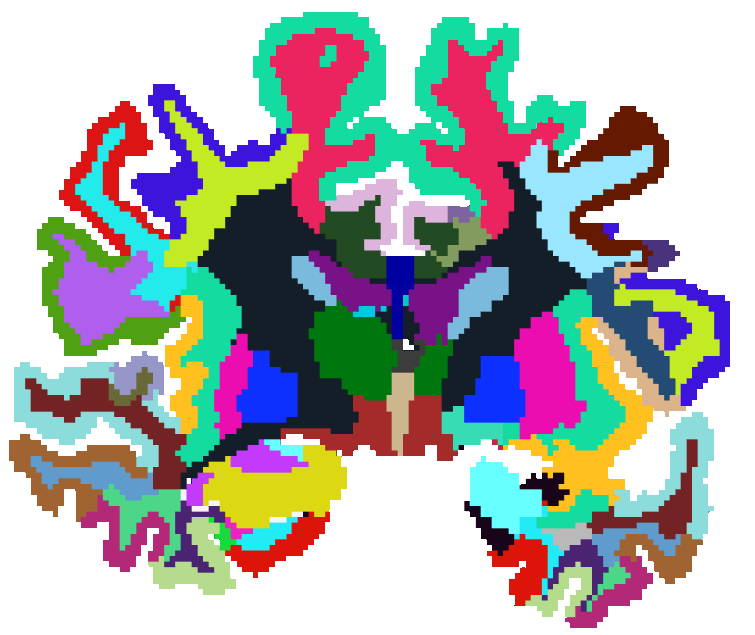
\includegraphics[height=4cm]{./chapters/chp4/FIG/parcellation-coronalwhiteBG_2.png}
  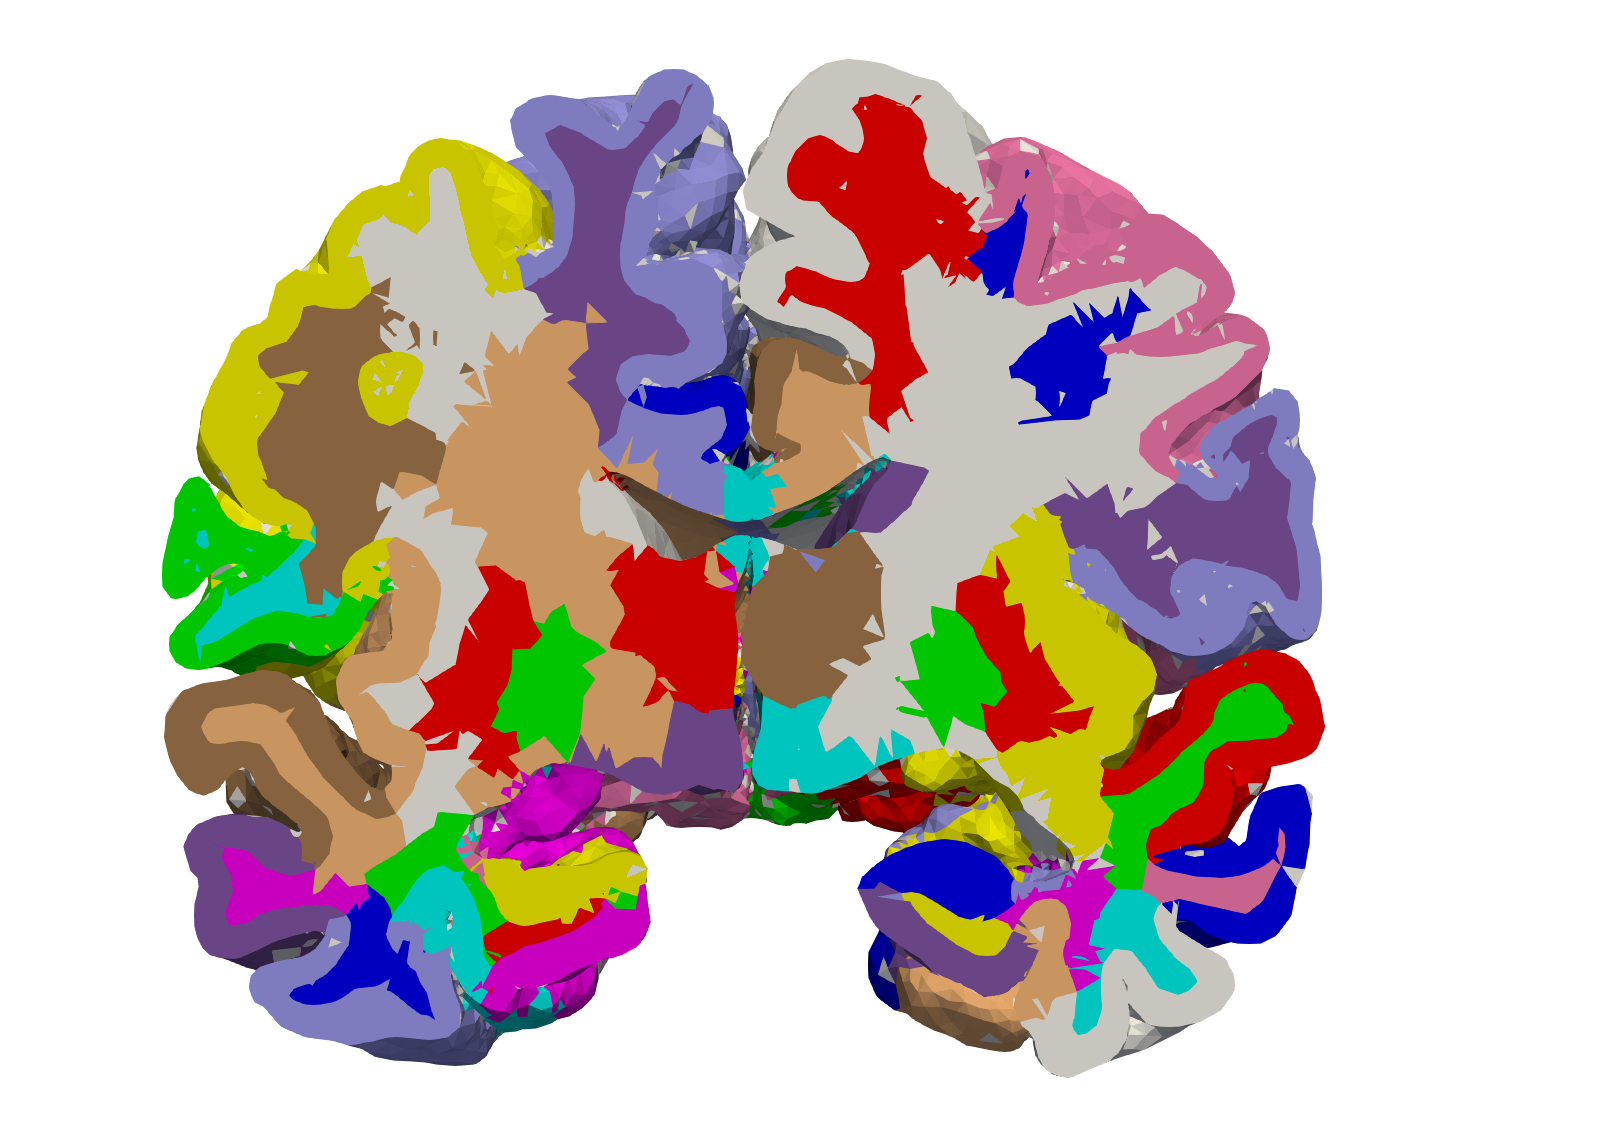
\includegraphics[height=4cm]{./chapters/chp4/FIG/ernie32-parcellation-basic.png}
  \caption{Brain parcellations. Left: Parcellation as generated
    by \freesurfer{} and visualized using Freeview. Right: Same
    parcellation transferred onto the FEniCS brain mesh and visualized
    using Paraview. (Different coloring, different slices, different view angles.)}
  \label{fig:chp4:freesurfer-parc}
\end{center}
\end{figure}

\subsection{Mapping a parcellation onto a finite element mesh}
\label{sec:chp4:mapping_parcellation}

In the brain parcellation, each region is identified by an integer
value. Our next goal now is to map these region tags onto the
generated volume mesh and into a FEniCS-compatible format. Doing so
involves:
\index{mesh data}
\begin{itemize}
\item
  reading and working with image (voxel-based) data in Python; 
\item
  representing discrete mesh data in FEniCS;
\item
  mapping values from voxel indices (voxel space) to mesh coordinates (RAS space).
\end{itemize} 
As usual, we will illustrate these steps using a concrete code example
(included in \emp{mri2fem/chp4/map\_parcellation.py}). We wrap our
main functionality in a Python function
\pythoninline{map_parcellation_to_mesh} taking the parcellation
filename and mesh filename as input (with \emp{wmparc.mgz} and
\emp{ernie-brain-32.xdmf} from the previous section as an example).
\newpythonsnippet{chp4}{map_parcellation.py}{64}{65}

\subsubsection*{Working with image data in Python}

\index{nibabel}
\index{FEniCS}
\index{NumPy}
We will use the Python packages NiBabel for working with neuroimaging
data, NumPy for general numerics in Python, and FEniCS for
representing the mesh and the mesh data:
\newpythonsnippet{chp4}{map_parcellation.py}{1}{4}

\noindent We begin by loading the image data from the parcellation
file as follows:
\newpythonsnippet{chp4}{map_parcellation.py}{6}{10}

\noindent We can e.g.~inspect the image shape (number of voxels in
each dimension): and extract voxel values by indexing the
\pythoninline{data} array:
\newpythonsnippet{chp4}{map_parcellation.py}{12}{15}

\subsubsection*{Representing discrete mesh data in FEniCS}

We aim to map these data onto the brain mesh generated from the same
T1 images. FEniCS offers the concept of a \emp{MeshFunction} for
representing such discrete data. Mesh functions can be associated with
cells, faces, edges or vertices. Here, we aim to identify the
parcellation region for each cell in the brain mesh and we will thus
make use of a cell function. We first import the full brain mesh:
\newpythonsnippet{chp4}{map_parcellation.py}{17}{21}

\noindent before creating a mesh function over mesh entities of
dimension 3 (cells) relative to it, with all entries initialized to 0:
\newpythonsnippet{chp4}{map_parcellation.py}{23}{27}
Note that the \emp{MeshFunction} can be indexed directly, or its values can be
accessed via the member function \emp{array}.

We now aim to iterate over all cells in the mesh (function), identify the
corresponding parcellation region and insert this value into the \emp{regions}
mesh function. However, at this point, a key question appears: we can
index the image data by its indices and the mesh by its cell or vertex
indices (and/or their coordinates), but how can we identify the voxel
index corresponding to a given cell or vertex (coordinate) and vice
versa? 

\subsubsection*{Converting between indices, coordinates and spaces}

\index{voxel space}
\index{RAS space}
Converting between voxel indices and other coordinates is a core
problem that we will encounter several times. To address this task, we
begin by introducing some nomenclature. The span of the image
dimensions is often referred to as the (T1) \emph{voxel space}, with
indices (or dimensions) $(i, j, k)$. On the other hand, the span of
the mesh axes defines the RAS (left-to-Right, posterior-to-Anterior,
inferior-to-Superior) space with coordinates $(x, y, z)$. We aim to
construct the transformation $f$ from voxel space to RAS space:
\begin{equation}
  (x, y, z) = f(i, j, k),
\end{equation}
as well as its inverse $f^{-1}$ from RAS to voxel space. Fortunately,
the parcellation information allows us to extract this transformation easily:
\newpythonsnippet{chp4}{map_parcellation.py}{29}{33}

We then iterate over the cells of the mesh, extract the cell index,
extract the RAS coordinates of the cell midpoint, convert from the RAS
coordinates to voxel space via a call to \emp{apply\_affine}, round
off to the nearest integer values to find the image indices and map
the corresponding image data value into the \emp{regions} mesh function:
\newpythonsnippet{chp4}{map_parcellation.py}{35}{49}

We save the resulting mesh function in XDMF format (suitable for
Paraview) or in the HDF5 format (suitable for further FEniCS processing). 
\newpythonsnippet{chp4}{map_parcellation.py}{51}{62}
The result can be seen alongside the original parcellation in
Figure~\ref{fig:chp4:freesurfer-parc}.

%% \begin{figure}
%%   \caption{Illustration of voxel and RAS space. Graphics}
%% \end{figure}

\subsection{Mapping parcellations respecting subdomains}
\label{chp4:parcellations}

By careful inspection of the mesh-based representation of the
parcellation in Figure~\ref{fig:chp4:freesurfer-parc} (right), we find
some artifacts in the labeling of the cells. Indeed, as the finite
element mesh is not aligned with the segmentation, the previous direct
mapping between cell midpoints and voxels can lead to minor
inaccuracies. In this section, we therefore aim to improve on our mesh-based
parcellation representation by using subdomain
information. 


Concretely, we aim to do the following
\begin{itemize}
\item
  Read a mesh with subdomain information such as gray and white matter
  regions;
\item
  Iterate over the cells in each subdomain separately, and calibrate
  voxel values against those of neighboring cells;
\item
  Store subdomain and parcellation information together.
\end{itemize}

\subsubsection*{Converting meshes and mesh data between different formats} 
\label{chp4:meshio-converting}

\index{meshio}
\index{mesh formats}
In Chapter~\ref{sec:chp4:tools:gray-white}, we created a mesh with
gray and white matter labels stored as subdomain information in the
.mesh format. Our first next step is to convert this information to a
FEniCS-compatible format. We will write a convenient Python for this
common operation, and use the opportunity to illustrate the use of an
\pythoninline{ArgumentParser} to read in arguments from the command
line instead of coding the arguments directly into the script
(included in \emp{mri2fem/chp4/convert\_to\_dolfin\_mesh.py}).

We begin by importing the relevant Python packages: \emp{argparse},
\emp{meshio} and \emp{dolfin}:
\newpythonsnippet{chp4}{convert_to_dolfin_mesh.py}{1}{3}

\noindent Our argument parser set-up looks like this:
\newpythonsnippet{chp4}{convert_to_dolfin_mesh.py}{53}{59}
\noindent and we then  call two functions (described below): 
\newpythonsnippet{chp4}{convert_to_dolfin_mesh.py}{61}{63}
The script can then be called as e.g.
\terminal{\$ cd mri2fem/chp4\\
\$ python convert\_to\_dolfin\_mesh.py -{}-meshfile ernie-gw.mesh -{}-hdf5file ernie-gw.h5}

We use meshio to first read the .mesh file, its data associated with
the mesh cells (\pythoninline{subdomains}), and its data associated with mesh
facets (\pythoninline{boundaries}). We then write these in the FEniCS-readable
.xdmf format as separate files.
\newpythonsnippet{chp4}{convert_to_dolfin_mesh.py}{5}{27}

Subsequently, FEniCS can read the .xdmf files into a
\pythoninline{Mesh} and \pythoninline {MeshFunction}s, and write these
collectively to a single .h5 file.
\newpythonsnippet{chp4}{convert_to_dolfin_mesh.py}{29}{51}

These can be read back into FEniCS as follows (with the filename given in \pythoninline{hdf5file}):
\newpythonsnippet{chp4}{add_parcellations.py}{36}{46}

\subsubsection*{Masking data and improved parcellation identification}

Let us now assume that we have available the \emp{mesh},
\emp{subdomains}, as well as the image \emp{data} from the
parcellation file (e.g \emp{wmparc.mgz}) and RAS to voxel space
transform \emp{ras2vox} as described in
Chapter~\ref{sec:chp4:mapping_parcellation}. Our next steps are to:
\begin{itemize}
\item
  find the RAS coordinates of all cell (midpoints), and map these to
  voxel space indices;
\item
  map parcellation values to mesh cells in a manner that ensures that
  parcellation regions do not extend across subdomains.
\end{itemize}
In particular, for each mesh cell, we will now examine a neighborhood of
corresponding voxel values to pick the most frequent adjacent one as
the matched parcellation value. 

We first extract all the RAS coordinates of the cell midpoints:
\newpythonsnippet{chp4}{add_parcellations.py}{57}{59}
before converting these to voxel coordinates and indices as before:
\newpythonsnippet{chp4}{add_parcellations.py}{68}{72}

We create a convenient map from voxel indices to subdomain tags, and
the \pythoninline{regions} array to be filled:
\newpythonsnippet{chp4}{add_parcellations.py}{74}{81}

We iterate over each subdomain separately, examine the voxel data
associated with this subdomain only, and for each cell determine the most
common tag in a neighborhood around its voxel:
\newpythonsnippet{chp4}{add_parcellations.py}{83}{96}
We can then update the subdomains array
\newpythonsnippet{chp4}{add_parcellations.py}{99}{104}
and store the resulting mesh data again:
\newpythonsnippet{chp4}{add_parcellations.py}{106}{111}

The \pythoninline{adjacent_tag} function reads as:
\newpythonsnippet{chp4}{add_parcellations.py}{7}{30}

The complete script is included in
\emp{mri2fem/chp4/add\_parcellations.py} and can be tested e.g. via:
\terminal{\$ python3 convert\_to\_dolfin\_mesh.py -{}-meshfile ernie-brain-32.mesh -{}-hdf5file ernie-brain-32.h5\\
  \$ python3 add\_parcellations.py -{}-in\_hdf5 ernie-brain-32.h5 -{}-in\_parc wmparc.mgz -{}-out\_hdf5 results/ernie-brain-subdomains-tags.h5 -{}-add 17 1028 1035 3028 3035
}

\section{Refinement of parcellated meshes}
\label{sec:chp4:addparcellations}

We end this chapter by examining how we can refine the generated
meshes and in particular how we can refine local regions. FEniCS
supports global and local mesh refinement and adaptivity through the
functions \pythoninline{refine} and \pythoninline{adapt}. The latter
(\pythoninline{adapt}) is particularly useful for refining mesh
functions and associated mesh data in addition to the refinement of
the mesh itself. The code snippets presented here are included in
a complete context in \emp{mri2fem/chp4/refine\_mesh\_tags.py}. 

\subsection{Extending the Python interface of DOLFIN/FEniCS}

DOLFIN, the problem-solving interface to FEniCS, provides a C++ and a
Python interface. The Python interface is generated from the C++
interface using pybind11, but the entire C++ API is not
exposed. Instead, a user can generate their own Python-bindings fairly
easily. As parts of the \pythoninline{adapt} interface is not by
default available in Python, we illustrate how to use pybind11 to
compile our own FEniCS wrappers here.

\index{pybind}
\index{Python wrappers}
Below, we provide Python bindings for the \emp{adapt} function. We
also notice that this function is overloaded and that we provide
bindings to six versions with different signatures. After the code is
executed, the bindings are compiled in to Python module. However,
notice that the module will not be added to the DOLFIN library, but
resides in the user's local cache.
\newpythonsnippet{chp4}{refine_mesh_tags.py}{6}{26}

\subsection{Refining certain regions of parcellated meshes}

Let's assume that, in Python, we have a FEniCS \emp{mesh} with FEniCS
mesh functions \emp{subdomains} and \emp{boundaries}, for instance
extracted from an .h5 file as illustrated in
Chapter~\ref{chp4:parcellations}. 

One option is then to refine the mesh globally, meaning that we refine
all cells of the mesh. We would then also like to refine or adapt the
associated mesh functions to the refined mesh. We can accomplish this
as follows:
\newpythonsnippet{chp4}{refine_mesh_tags.py}{43}{56}

\begin{figure}[t]	
  \begin{center}
    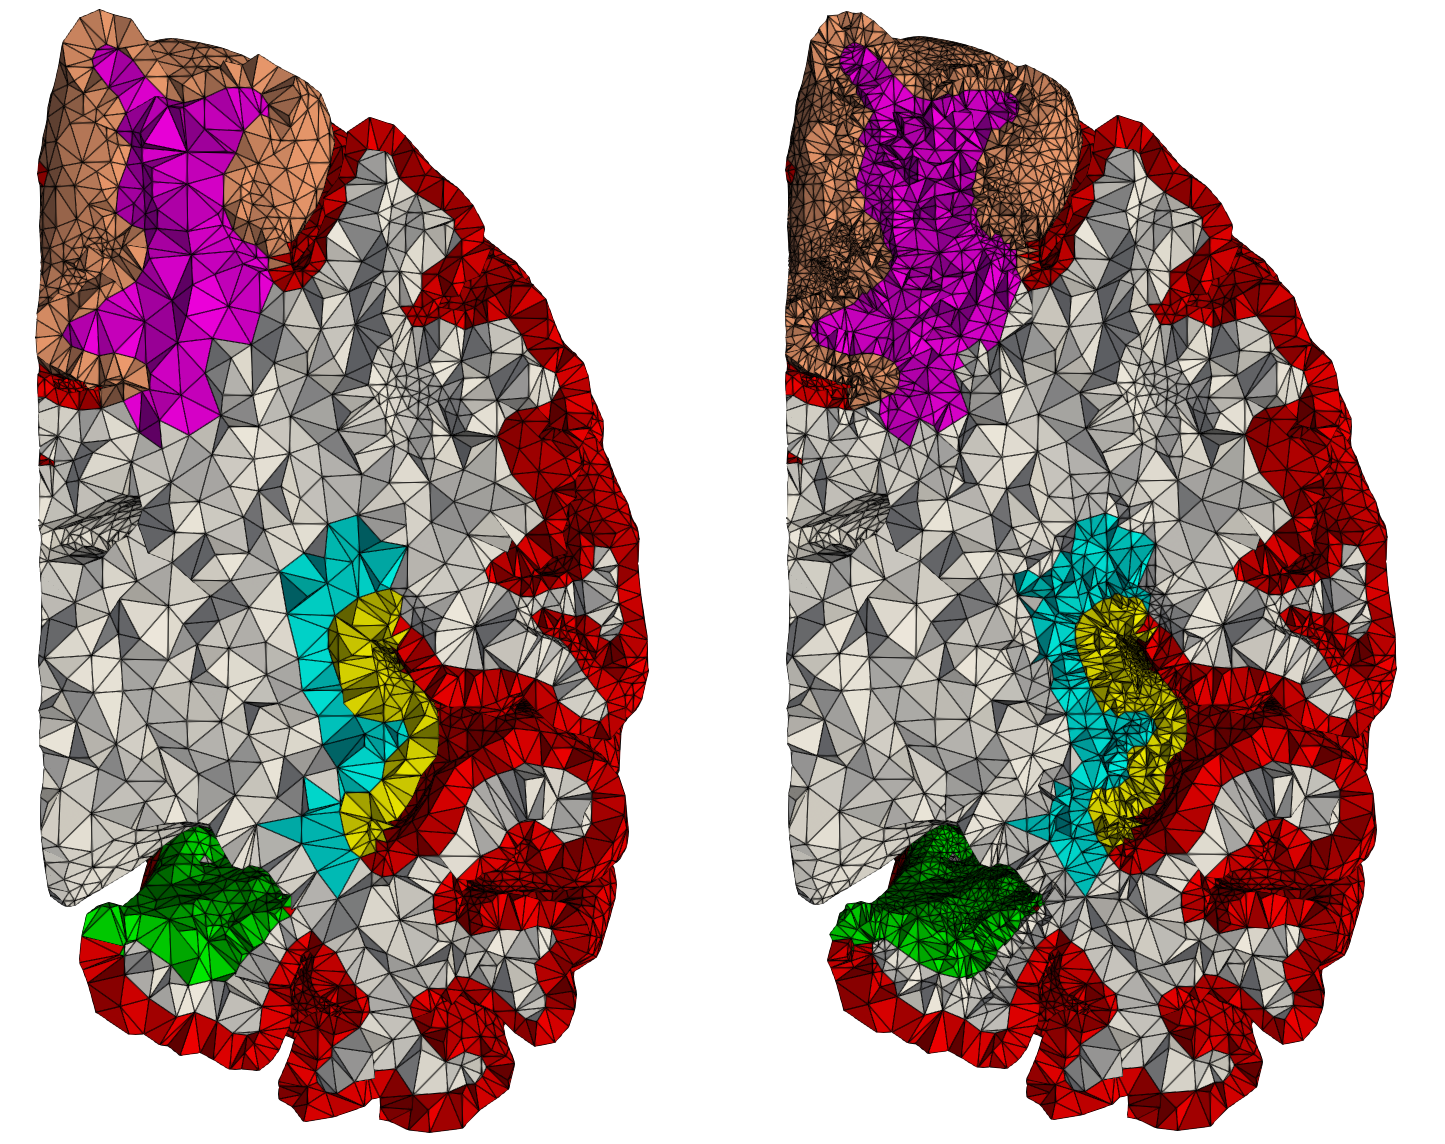
\includegraphics[width=0.7\textwidth]{./chapters/chp4/FIG/fenics-parcellation-crinkle.png} \\
    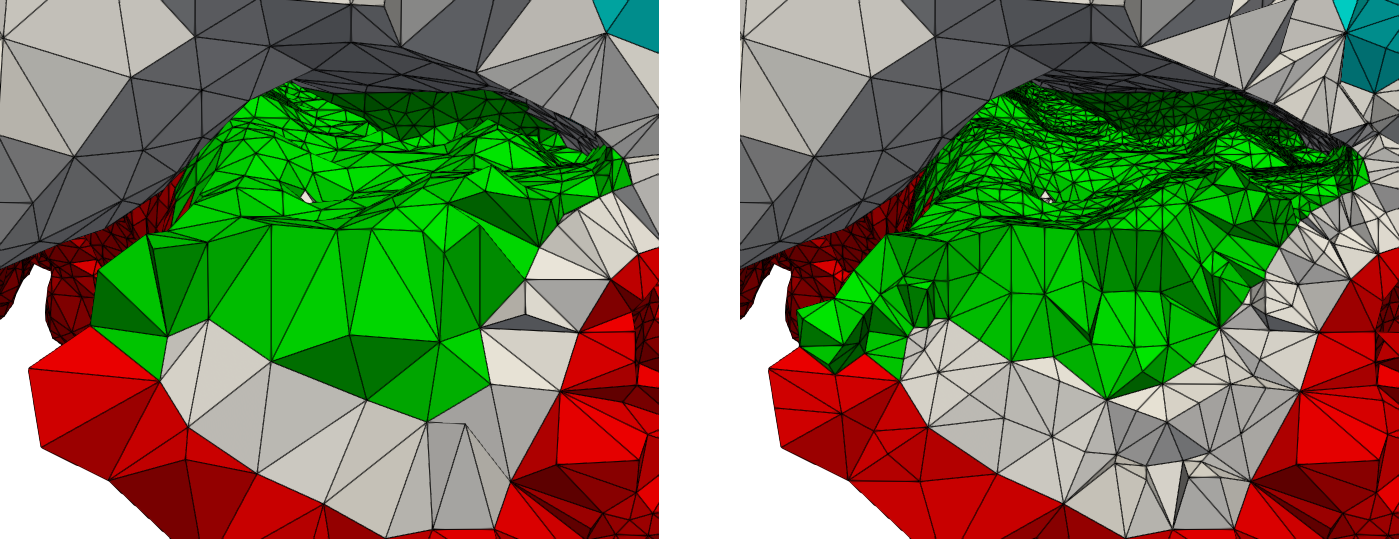
\includegraphics[width=0.9\textwidth]{./chapters/chp4/FIG/parcellations_refine_zoom.png}
  \end{center}
  \caption{Illustration of left hemisphere meshes with different
    parcellation regions at different resolutions. The meshes on the
    right are local refinements of the meshes on the left. Zoom of the
    hippocampus region (green).}
  \label{fig:chp4:fenics-parc}
\end{figure}
Alternatively, we can refine the mesh locally. In order to do so, we
provide the adapt function with a boolean cell-based mesh function
that sets each mesh cell as a candidate for refinement (\emp{True}) or
not -- unless as a side effect of the refinement algorithm
(\emp{False}). Assuming that we have a list \emp{tags} with the
subdomain tags for e.g. parcellation regions that we would like to
refine, we consider:
\newpythonsnippet{chp4}{refine_mesh_tags.py}{58}{73}
Local refinement of a mesh with labeled parcellation regions is
illustrated in Figure~\ref{fig:chp4:fenics-parc}.

